\chapter{Analysis and Results}


\section{2022 vdM scan program}

The main VdM scan program for the CMS experiment was performed in November 2022 during LHC fills 8379 and 8381. In fill 8381 on 10 and  11 Nov 2022 at pp collision energy $\sqrt{s}$ of 13.6 TeV  144 bunch pairs were colliding at the CMS intertion points at zero crossing angle, with two additional unpaired bunches present in each beam. Four VdM scan pairs, two beam-imaging (BI) scan pairs and one length scale scan pair where performed, where each scan pair consists of two scans in the transverse planes x and y, as well as other scan types not included in this analysis. In a VdM scan, the two beams are separated by $6\sigmab$ ≈ 578 $\mu m$ and scanned across one another in a sequence of 25 steps of 30 s with a step size of $0.5\sigma_{b} \thickapprox 48 \mu m$, where $\sigma_{b}$ is the transverse bunch size. In the BI scans, one beam is kept fixed at its nominal head-on position while the other is separated and scanned in 19 steps of 46 s from $-4.5\sigma_{b}$ to $+4.5\sigma_{b} \thickapprox 433 \mu m$. In a length scale scan, the beams are separated by a constant amount of $\sqrt{2} \sigma_{b} \thickapprox  106 \mu m$  and moved coherently forward and backward in five steps each in the same transverse direction, finally two super separation periods were performed for the analysis and Background sustraction, here the two beams were sepated at a distance of $6\sigma$.  The scan program during fill 8381 is summarized in Fig. \ref{scan_prog}.\\

The VdM calibration itself is based on scans recorded during the fill 8381, where the  Six scan pairs using for  this analysis were performed, they are labeled consecutively as they were recorded in time, as “VdM1”, “BI1”, “BI2”, “VdM2”, “VdM3”, and “VdM4” as shown in figure \ref{scan_prog} . During the "VdM2" scan pair, the central CMS data taking was not operational, so no data was recorded for PCC, and this scan pair is skipped in the PCC VdM analysis. To ensure a dataset with a high event count for PCC even at large beam separations, CMS gated the zero-bias triggers on 5 bunch pairs: BCIDs (Bunch Crossing ID) 282, 822, 2944, 3123, and 3302 and recorded events with a total rate of 27.23 kHz.\\

\begin{center}
  \begin{figure}[h]
    \centering
    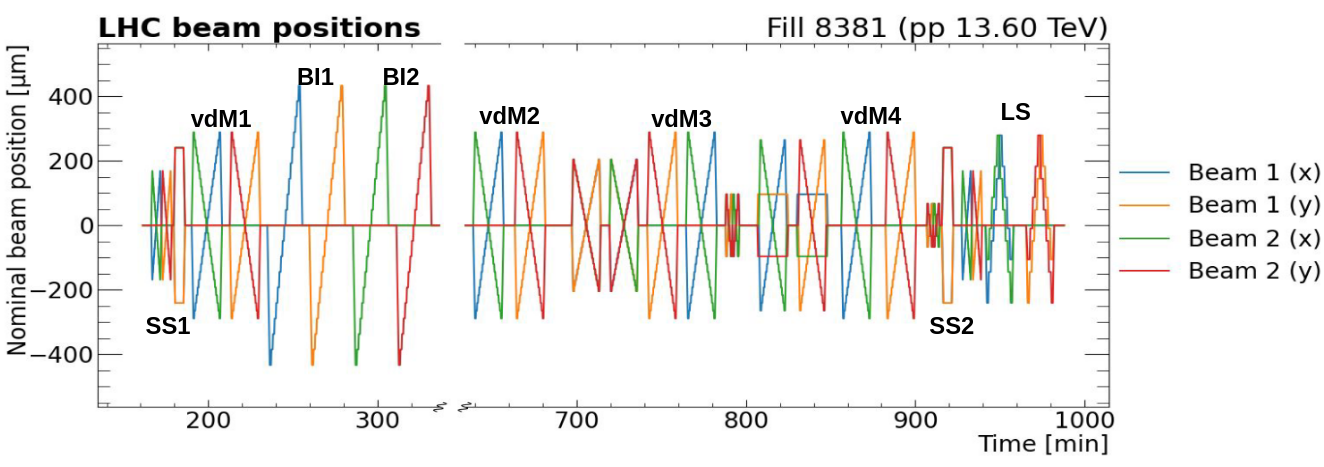
\includegraphics[scale=.25]{Chapter4/2022Scanprorgam.png}
    \caption[2022 scan program]{Nominal horizontal and vertical positions of the proton beams during LHC fill 8381, showing the four normal VdM scans, two BI scans and the two Super Separation Periods (SS)}
    \label{scan_prog}
  \end{figure}
\end{center}

The rate measured by each detector and normalized with the measured beam population is
fitted as a function of the separation. Corrections to the measured proton numbers and to
the nominal separation are discussed in the following sections. Here, the fit model and the
background subtraction are discussed. Technically, the fits are performed with the VdMFramework.

%CMS BRIL Project, “VdMFramework documentation”. CMS Website, 2023.
%https://vdmdoc.docs.cern.ch/.

%For the background estimation, two Super Separation (SS) periods were carried out during the scan program, each 5 minutes long where the beams were separated by $6\sigma_{b}$ (where $\sigma_{b}$ the beam size) in both the x and y directions.

\section{Data analysis}

The data taken by the  PCC luminometer was reprocessed for the CMS team to perform a cluster reconstruction. The datasets containing the cluster information per event were stored in 16 different "zero Bias" datasets. The first step we took was to extract the data corresponding to the events that belong to our 6 VdM Scans (Runs, Pixel cluster clusters, timestamps, etc.) in a file with ROOT format that is the CERN's data analysis package. This was done through the CMS software (CMSSW), which is written in Python2 and C++.\
Afterward, we have the 16  resuulting datasets, uno for each "zero Bias" dataset. These files are reprocessed to generate the final file containing the rates stored per 1.32 s (NB4) with a hierarchical data format (HD5). Within this data reprocessing, we clean the information by subtracting the background and also select the modules that were previously analyzed by a stability study.

The final "hd5" file containing the rates from the detector with data collected during the vdM scans is analyzed using a software framework called the "vdM Framework" (vdM FW), which is the latest version and is written in Python3. The vdM FW uses data analysis package, "ROOT," through the "PyRoot" library. With the analysis and plotting tools, the vdM FW reads the hd5 file, producing several intermediate files: scan file, beam currents file, rates file, and correction files. It then applies corrections to the rates (Background, DynamicBeta), separation (OrbitDrift, LengthScale, BeamBeam), and creates a graph file. This graph file contains the normalized rates (i.e., $R/N_{1}N_{2}$) and beam position. Each point corresponds to the averaged rates in a time window of 30s and 46s for vdM scans and BI scans, respectively. The points are then fitted with a predefined function to extract $\Sigma_{x,y}$ and peak values to compute $\sigma_{\text{vis}}$ for all the bunches in the scan.

\section{Background estimation}

To extract $\Sigma_{x,y}$ through fitting, it is necessary to correct the raw measured rates for background in the detector beforehand. The background contribution is estimated independently during the Super Separation (SS) period comented in the above section. During this period, the beams are separated by $6\sigma_{b}$, ensuring that the only contribution is from background. There are three principal sources of beam-induced background to consider:

\begin{itemize}

\item Beam Gas Elastic (BGE). The elastic beam gas contribution are all coherent and quasi-elastic nuclear elastic and coulomb scattering for multi-turn beam-gas interactions around the ring. Typically the interaction of the primary beam proton and the takes place at the TCT collimator, so that this background contribution has an almost point- like source \cite{bkg_source}.

\item Beam Gas Inelastic (BGI). These are all inelastic interactions of primary beam protons with rest gas in the beam pipe. The interaction rate is dominated by the vacuum quality in the various beam line elements upstream CMS. Therefore the origin of this contribution is distributed all along the long straight section \cite{bkg_source}.

\item Beam Halo (BH). This component of the machine induced background is caused by the inefficiency of the main collimation system. Protons can escape from one collimator and being intercepted by another collimator \cite{bkg_source}.
\end{itemize}

In order to illustrate the two SS periods for this analisys, Figure \ref{ssp_wide_bx282} displays the PCC per NB4 versus time for BCID 282. The lower regions of the plot correspond to a time window of 5 minutes during which the beams were separated by a distance of $6\sigma_{b}$.\\

\begin{center}
\begin{figure}[h!]
\centering
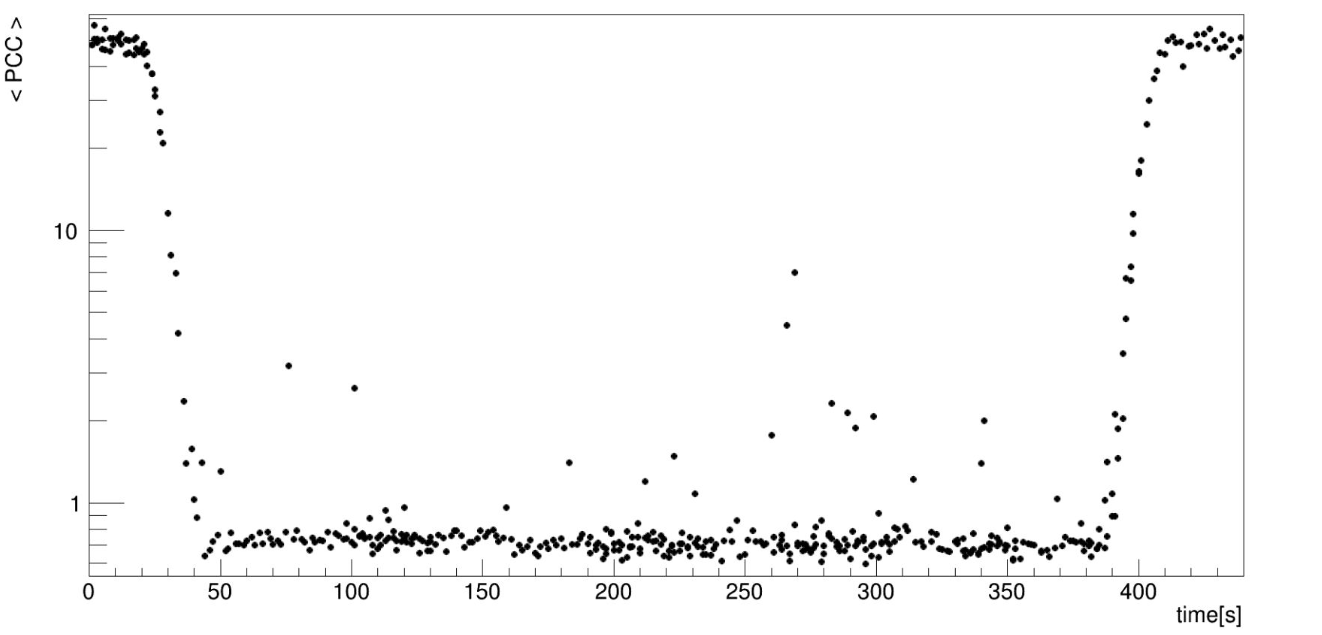
\includegraphics[width=.49\textwidth]{Chapter4/BX_282_Rates_SS1.png}
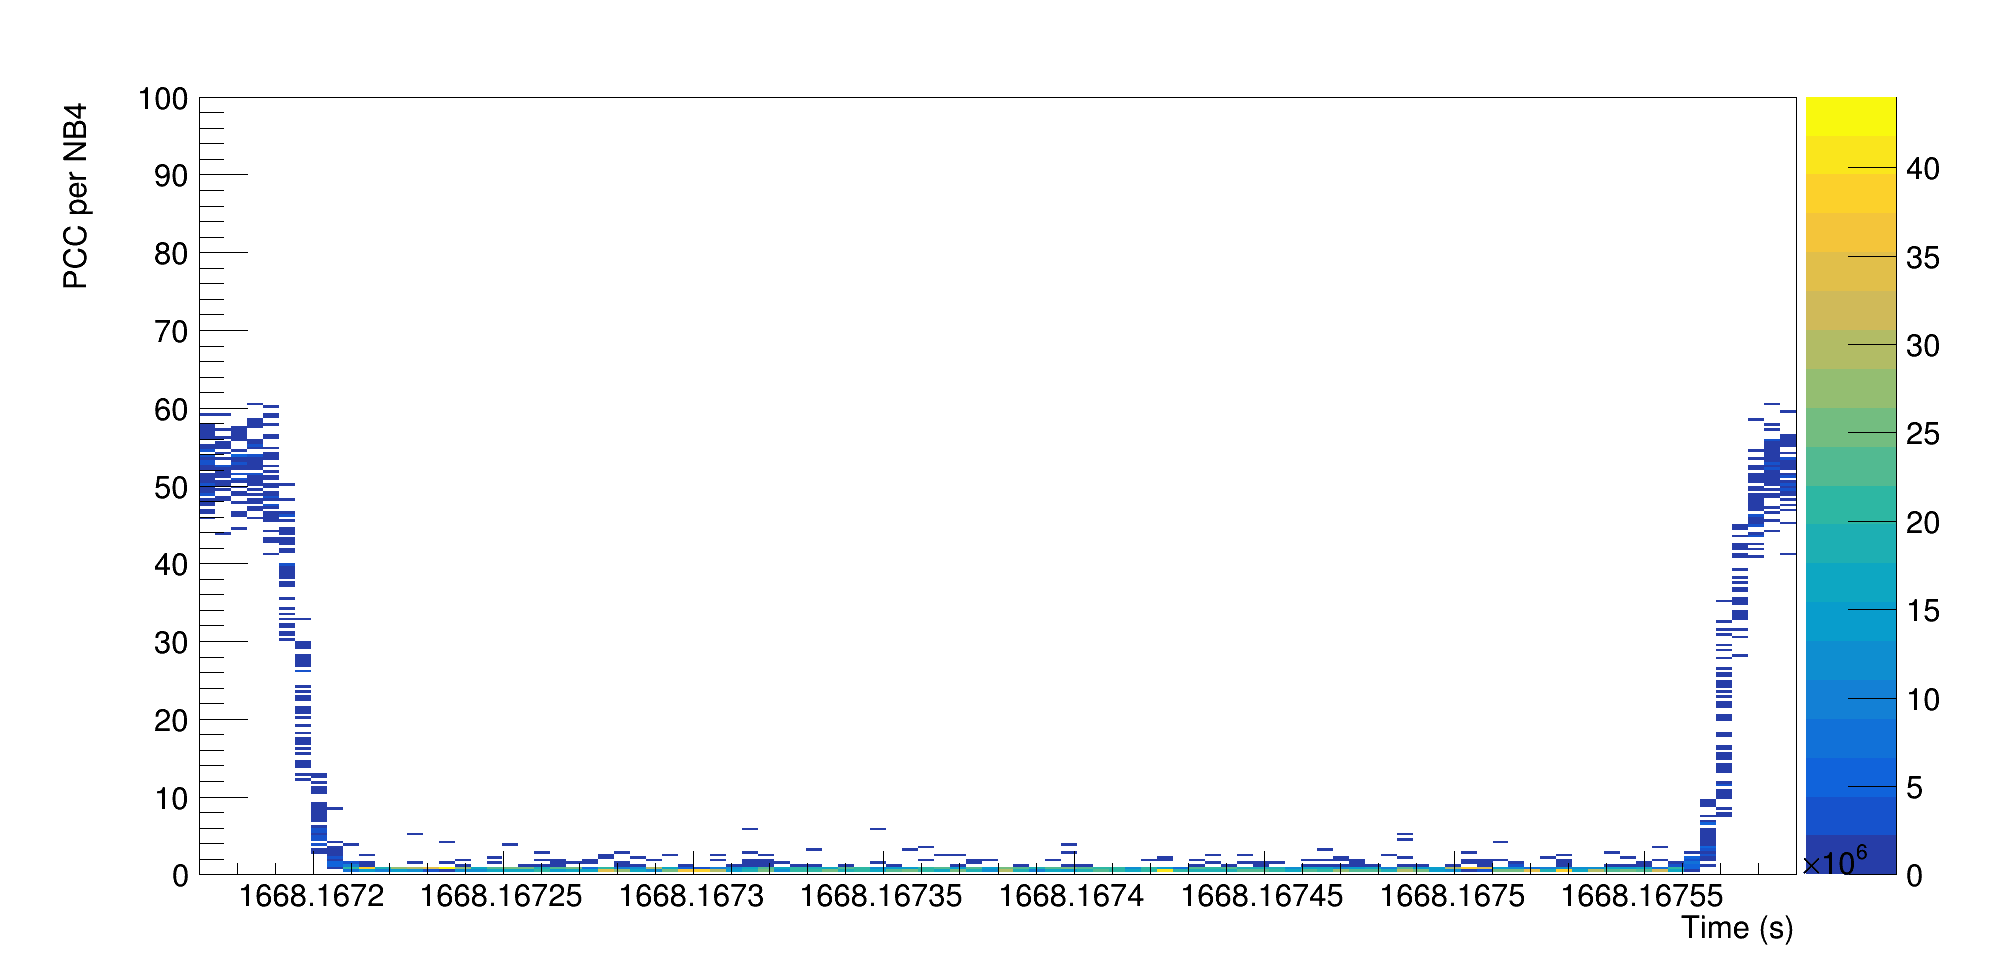
\includegraphics[width=.49\textwidth]{Chapter4/BX_282_Rates_SS2.png}
\caption[Super Separation periods for BCID 282]{PCC per NB4 versus time for BCID 282. The lower regions corresponds to the super separation period I (left) and II (right).}
\label{ssp_wide_bx282}
\end{figure}
\end{center}

To estimate the background value in each BCID, the mean value of the PCC per NB4 rates distribution is computed. The mean and error per super-separation (SS) period are obtained by plotting the PCC per NB4 as a function of time and then taking the y projection. The error is calculated using the formula $AvgErr = \sqrt{SEM_1^2 + SEM_2^2 + \cdots + SEM_N}/N$. To illustrate this process for each BCID, the distribution or profile of PCC per NB4 for each SS period is plotted. Figure \ref{ss1_hist_282} displays the PCC per NB4 distribution for SS period I specifically for BCID 282, but the same plot is created for every BCID.\\

\begin{center}
  \begin{figure}[h!]
    \centering
    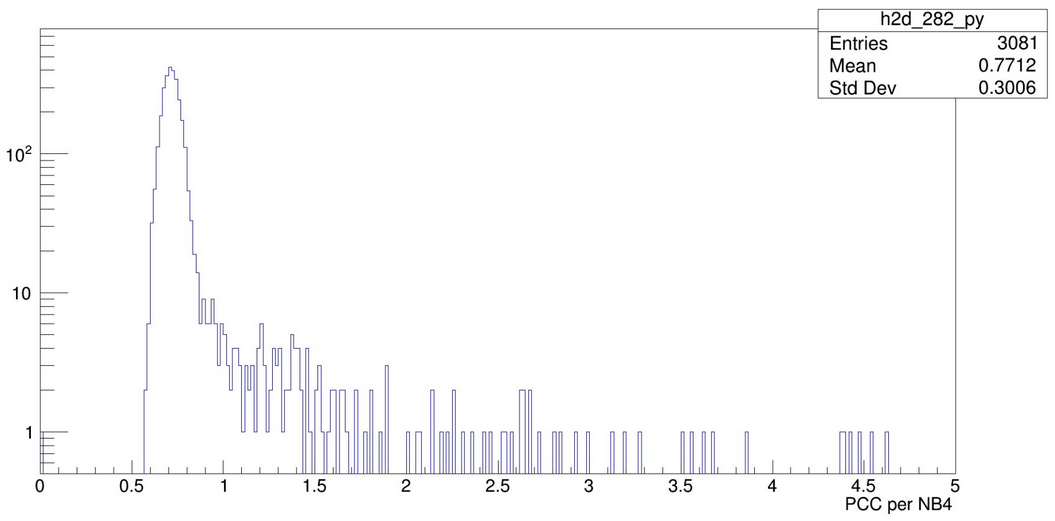
\includegraphics[scale=.18]{Chapter4/ss1_histo_bx282.png}
    \caption[PCC per NB4 profile for BCID 282 from SS period I]{ PCC per NB4 profile for BCID 282 from SS period I.} 
    \label{ss1_hist_282}
  \end{figure}
\end{center}


\begin{table}[h!]
  \begin{center}
    \caption{Mean and standard error on mean (SEM) for the PCC background estimated with the SS1 and SS2 data, separately for all five BCIDs and averaged.}
    \label{ss_per_bx}
    \begin{tabular}{|c | c | c | }
      \multicolumn{1}{c}{} & \multicolumn{1}{c}{\textbf{SS period I}} & \multicolumn{1}{c}{}  \\
      \hline
 \textbf{BCID}   & \textbf{Mean}   &  \textbf{SEM}\\
     \hline %\midrule[1.1pt]
      282 & 0.7712 & 0.0054\\
      \hline
      822 & 0.7744 & 0.0055\\ 
      \hline
      2944 & 0.7695 & 0.0057\\ 
      \hline
      3123 & 0.7469 & 0.0049\\ 
      \hline
      3302 & 0.7708 & 0.0049\\ 
      \hline
      \multicolumn{1}{c}{} & \multicolumn{1}{c}{} & \multicolumn{1}{c}{}\\
      \multicolumn{1}{c}{$\text{SSI}_{\text{Avg}}=$} & \multicolumn{1}{l}{$0.7665 \pm 0.0023$} & \multicolumn{1}{c}{}\\
%      \multicolumn{1}{c}{} & \multicolumn{1}{c}{} & \multicolumn{1}{c}{}
    \end{tabular}
    \hspace{0.5cm}
    \begin{tabular}{|c | c | c | }
      \multicolumn{1}{c}{} & \multicolumn{1}{c}{\textbf{SS period II}} & \multicolumn{1}{c}{ }  \\
      \hline
 \textbf{BCID}   & \textbf{Mean}   &  \textbf{SEM}\\
     \hline %\midrule[1.1pt]
      282 & 0.7192 & 0.0048\\
      \hline
      822 & 0.7257 & 0.0057\\ 
      \hline
      2944 & 0.7292 & 0.0058\\ 
      \hline
      3123 & 0.7028 & 0.0052\\ 
      \hline
      3302 & 0.7208 & 0.0053\\ 
      \hline
      \multicolumn{1}{c}{} & \multicolumn{1}{c}{} & \multicolumn{1}{c}{}\\
      \multicolumn{1}{c}{$\text{SSII}_{\text{Avg}}=$} & \multicolumn{1}{l}{$ 0.7195 \pm 0.0024$} & \multicolumn{1}{c}{}
    \end{tabular}   
  \end{center}
\end{table}

Table  \ref{ss_per_bx} shows the results for five different BCIDs, using the reprocessed PCC data for Fill 8381.  The overall background correction applied to raw PCC rate is $0.74305 \pm 0.002407$, which is calculated by taking the average of the mean values of SS1 and SS2. 

\section{Corrections}

There are several systematic effects that affect the measurement of beam overlap width and therefore the extraction of $\sigma_{vis}$ from the VdM scan procedure. These effects are measured and, where applicable, corrected as described below. A systematic uncertainty is assigned to the resulting measured cross-section, and the following corrections are applied in the VdM Framework:
 
\begin{enumerate}

\item Ghost and Satellite. This correction corrects for the presence of ghost and satellite spurious charges, which affect bunch currents. Satellite charges refer to additional charges outside the actual colliding bunch, while spurious charges refer to charge not in any nominally filled bunch slot. These results in corrections of up to 0.5\% to $\sigma_{vis}$. The overall uncertainty in the bunch current measurement is estimated to be 0.4%.

\item Background. This refers to the noise in the detector where there are no collisions. This value, estimated above, is subtracted from the rates.

\item Orbit drift. The orbit drift correction accounts for potential movement of the LHC orbit during the VdM scans. Time-dependent changes of the transverse beam positions for fixed machine parameters can alter the beam separation. This correction is composed of two independent corrections: 

\begin{itemize}

\item Orbit drift separation "ODS", correction that aims to correct for the orbit drift in the scanning direction and only affects beam separation. 

\item  Orbit drift rate "ODR", correction that aims to correct for the orbit drift in the direction orthogonal to the scanning direction and only affects the luminometer rate. The derived correction assumes that the beam overlap has a single Gaussian shape. The correction reads the $\sigma_{vis}$ in the orthogonal direction from the previous correction. 
\end{itemize}

Applying this correction improves the agreement between the $\sigma_{vis}$ values derived with different scan pairs and changes the average $\Sigma_{vis}$ by about 0.3\%. The full size of the correction is considered as uncertainty.

\item Beam Beam corrections.  The electromagnetic interaction between the two colliding proton bunches leads to two ef- fects in beam-separation scans:

\begin{itemize}

\item Beam Beam deflection. Corrects Beam Beam deflection (BB) that happens during bunch crossings at the collision point.accounts for the electrical repulsion of the beams, which increases the lateral
separation  The deflection is calculated and added to the nominal separation.

\item Dynamic Beta. The so-called dynamic-$\beta*$ effect, which accounts for any changes in the proton density distributions of the bunches due to the single-particle interactions. As a result, the non-linear change during separation steps in transverse bunch profiles is observed, and can described by the effective change of the $\beta*$  value.
\end{itemize}
The corrections are calculated for each proton bunch pair individually, and the combined effect of the two corrections is an increase of σvis by 1.0\%, with an uncertainty of 0.5\%.

\item Length Scale.  It applies a linear scaling to the beam separation to convert it from the "CMS scale" to the actual "physics scale". This is  calibrated by analyzing pp collision vertices reconstruced by the CMS tracker using data from the five length scale scan pairs performed in fills 8178, 8379, and 8381.%Length scale factors of (−0.56 ± 0.08)\% in x and (−0.43 ± 0.10)\% in y are found. The quoted uncertainty accounts for the statistical uncertainty, 
This correction reduces $\sigma_{vis}$ by 1.0\% and results in an uncertainty of 0.12\%.

%https://gitlab.cern.ch/bril/VdMFramework/-/wikis/od-flag
\end{enumerate}

\newpage
\section{van der Meer Scans and $\sigma_{vis}$ Results}

In the previous section, inconsistencies were observed in the background values, which resulted in a very high chi-square value. Therefore, it was decided not to use background subtraction. Instead, a fitting function was used, which applies a constant to achieve optimal values in the fit and improve the chi-square. To correct the measurements of PCC, beam separation, and beam currents, the corrections mentioned earlier were applied. The implemented fit model is a double Gaussian function combined with a constant-like function refered as "DG+Const":

\begin{equation}
DG+Const=
 C+P \cdot \Biggl[ F \cdot \exp \Biggl( \frac{-(x-\bar{x})^{2}}{2 \sigma_{1}^{2} } \Biggr) + (1-F) \cdot \exp \Biggl( \frac{-(x-\bar{x})^{2}}{2 \sigma_{2}^{2} } \Biggr) \Biggr] 
\end{equation}

%\begin{equation}
%DG+Const=
 %C+P \cdot \Biggl[ F \cdot \exp \Biggl( \frac{-(x-\bar{x})^{2}}{2 ( \frac{\sigma_{1}}{F_{Ratio}+1-F})^{2} } \Biggr) + (1-F) \cdot \exp \Biggl( \frac{-(x-\bar{x})^{2}}{2 ( \frac{\sigma_{2}}{F_{Ratio}+1-F})^{2} } \Biggr) \Biggr] 
%\end{equation}
where $F$ is the weight between 0 and 1 of the first Gaussian in the sum, $x$ is the beam separation $C$ is the constant value, $P$ the peak rate, $\bar{x}$ the mean and $\sigma_{1,2}$ the standard deviations are fit parameters. Fig. \ref{vdM1_282_XYscan} shows the fitted graphs of the first vdM scan pair for BCID 282 where  all the corrections described in the previous section have been applied and where  rates are normalized by the beam currents, which is a factor of eq. \ref{sigmavis_eq}  ($R(0,0)/N_{1}N_{2}$).

\begin{center}
\begin{figure}[h!]
\centering
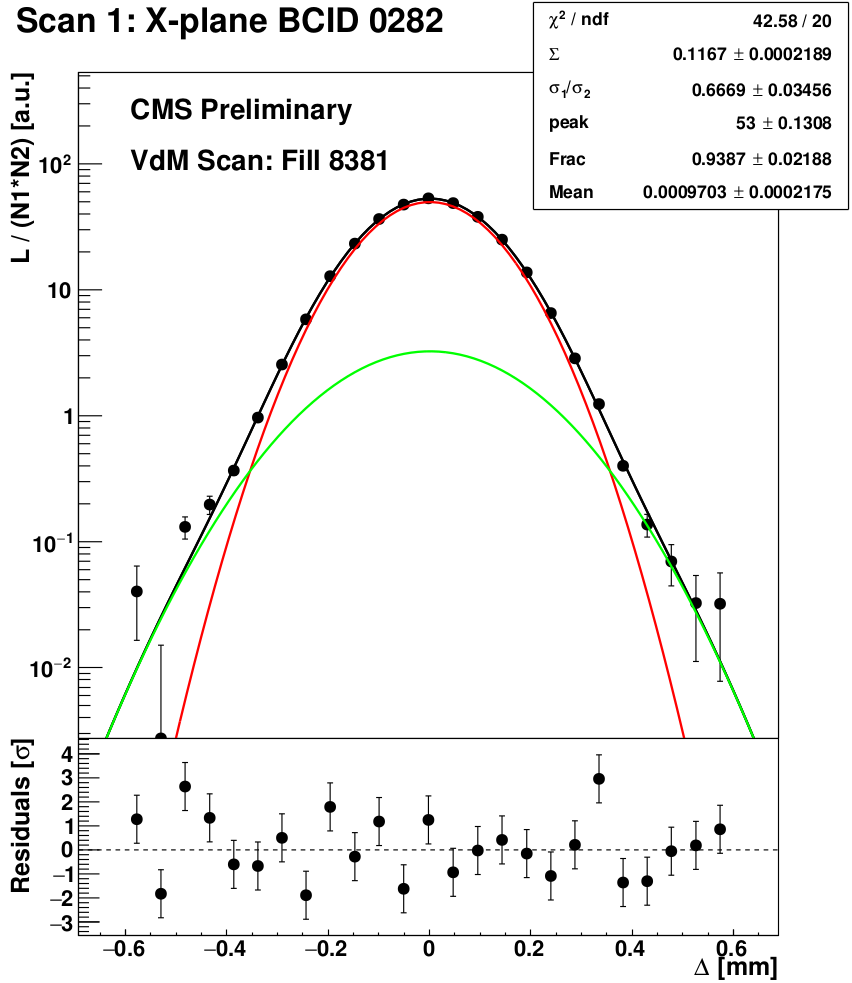
\includegraphics[width=.37\textwidth]{Chapter4/xscan.png}
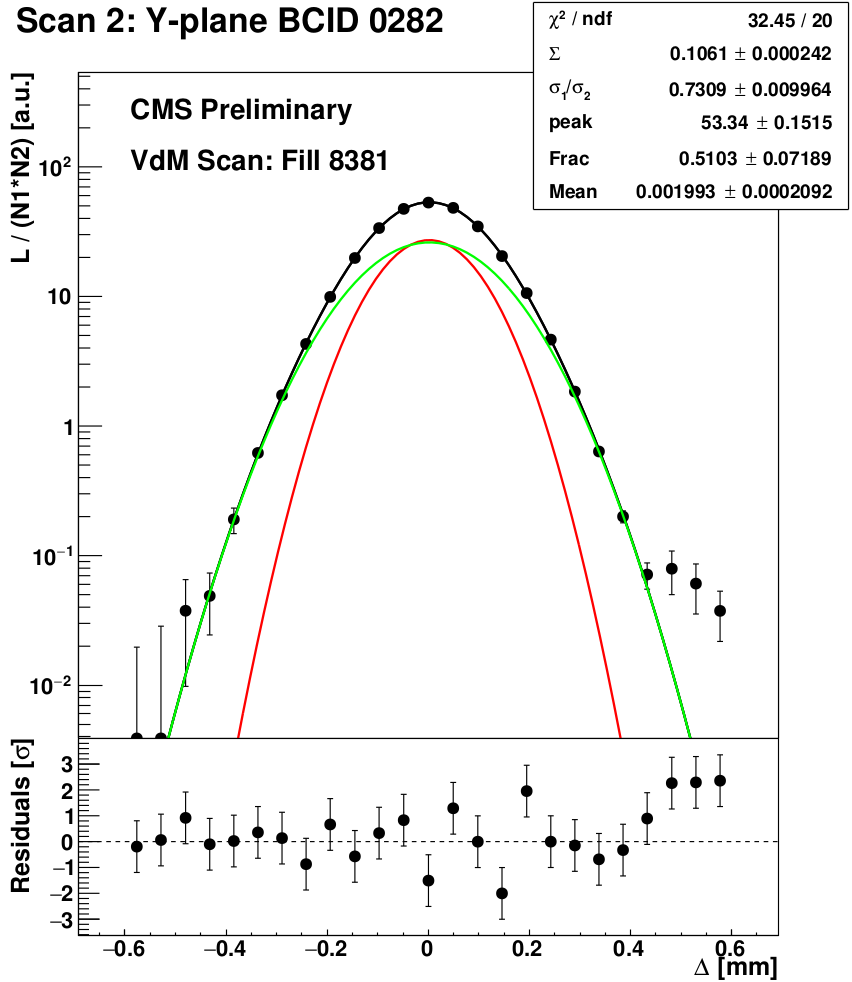
\includegraphics[width=.37\textwidth]{Chapter4/yscan.png}\\
\caption[vdM1 BCID 282]{Normalized rates and the resulting fitted curves with the DG+Const fit model as a function of the beam separation ($\Delta$) for BCID 282 for X (left) and Y (right) scan for the first vdM scan.}
\label{vdM1_282_XYscan}
\end{figure}
\end{center}

\newpage
For the remaining BCID's, the fits for both vdM and BI scans exhibit a very similar behavior, and in all cases, the fits have converged successfully. To evaluate the goodness of fit, Fig. \ref{chi2/ndof} displays a plot of the chi2/ndof for all the five scan pairs, which has a mean value of 1.88.
To compute $\sigma_{vis}$, the CapSigma $\Sigma_{x,y}$ and peak values have been extracted from the fits. Fig. \ref{capsigma_peak} presents the $\Sigma_{x,y}$ and peak values for all scan pairs. The plot clearly illustrates that both values reflect the fact that beam size increased over time in the $x$ dimension and decreased over time in the $y$ dimension.

\begin{center}
  \begin{figure}[h!]
    \centering
    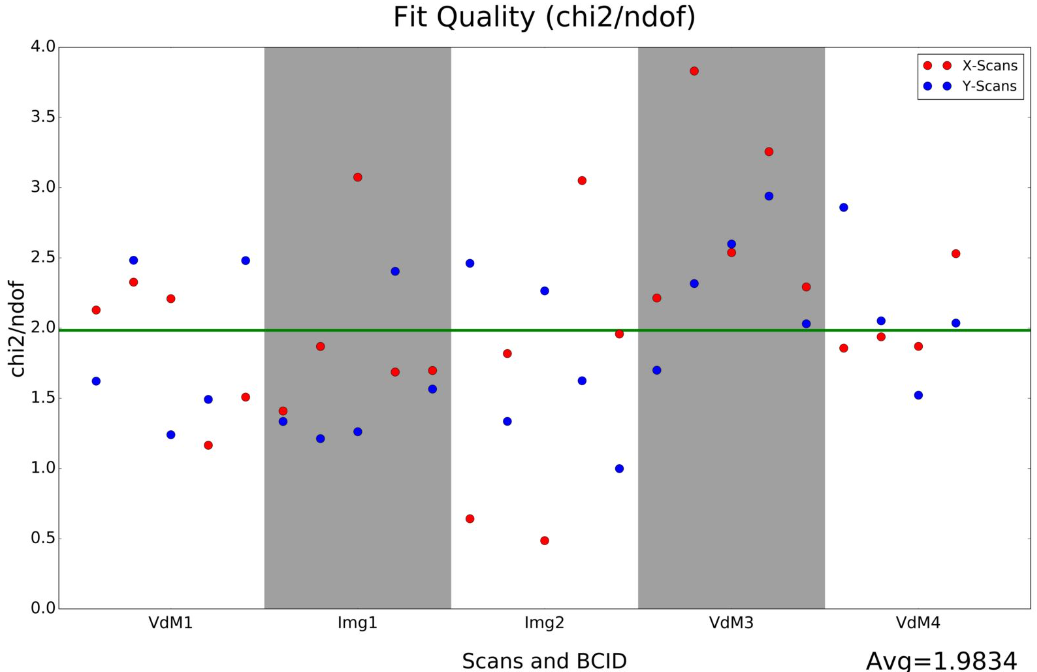
\includegraphics[scale=.03]{Chapter4/DGConst_chi2.png}
    \caption[chi2/ndof for all scan pairs]{ chi2/ndof for all the scan pairs.  where the red dots represent the X scans, and the blue dots represent the Y scans. It is important to note that in each scan, the BCIDs follow the same order, which is 282, 822, 2944, 3123, and 3302.} 
    \label{chi2/ndof}
  \end{figure}
\end{center}

\begin{center}
  \begin{figure}[h!]
    \centering
    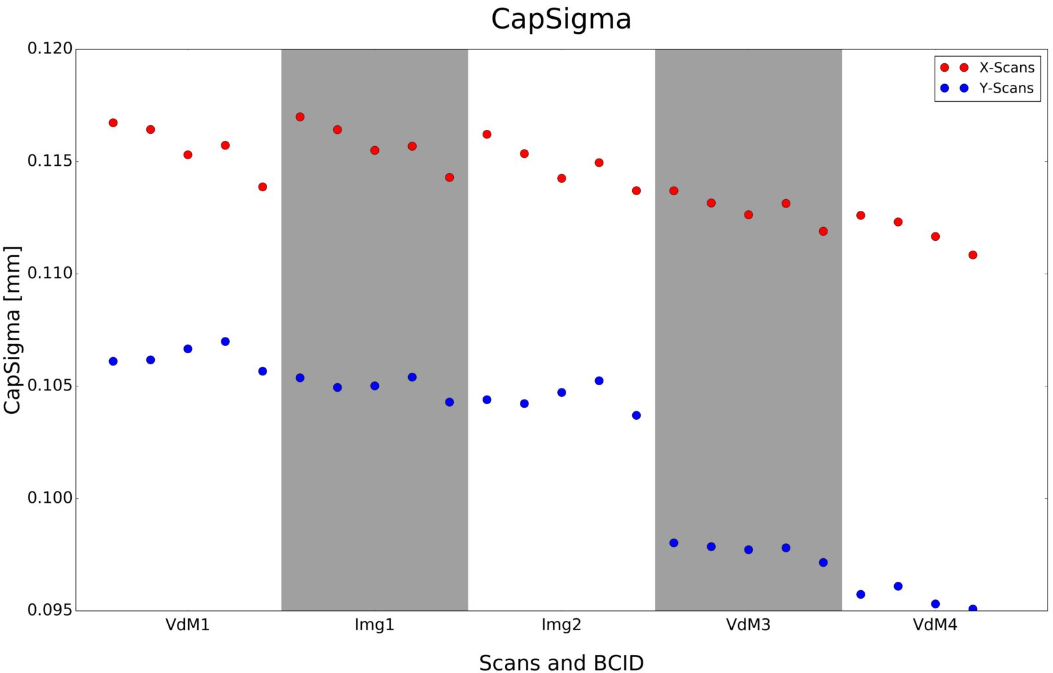
\includegraphics[width=.49\textwidth]{Chapter4/DGConst_CapSigma.png}
    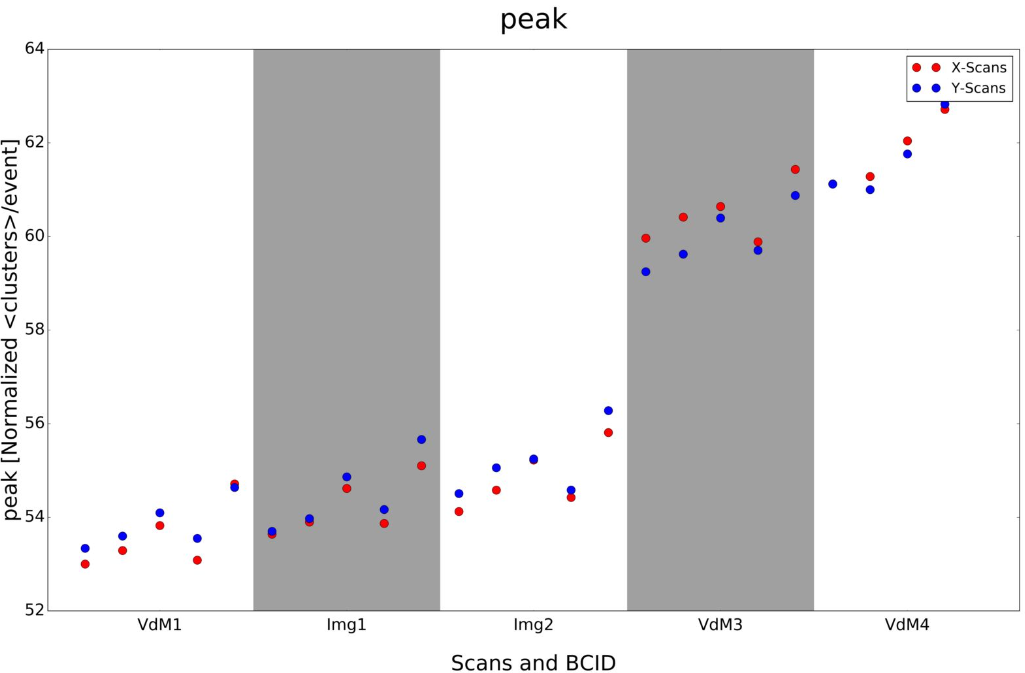
\includegraphics[width=.48\textwidth]{Chapter4/DGConst_peak.png}
    \caption[$\Sigma_{x,y}$ and peak values for all scan pairs]{$\Sigma_{x,y}$ (left) and Peak values (right) extracted from the fitted graph to compute $\sigma_{vis}$, where the red dots represent the X scans, and the blue dots represent the Y scans, note that in each scan, the BCIDs follow the same order, which is 282, 822, 2944, 3123, and 3302.} 
    \label{capsigma_peak}
  \end{figure}
\end{center}

The sigma visibe $\sigma_{vis}$ for all BCID's (vdM a BI acans) is computed from the fit results parameters Capital sigma $\Sigma_{x,y}$ and $peak_{x,y}$, this is done using the equation \ref{sigmavis_eq}. The value of $R(0,0)$ is obtained by taking the average of the peaks in the x and y directions ($R(0,0)=(Peak_{x}+Peak_{y})/2$), which have already been normalized, so \ref{sigmavis_eq} is rewritten as:

\begin{equation}
 \sigma= 2\pi \Sigma_{x} \Sigma_{y} \Biggl( \frac{Peak_{x}+Peak_{y}}{2} \Biggl)
 \end{equation}
 
Fig \ref{sigmavis_perbcid} shows the  value of sigma visible $\sigma_{vis}$ per BCID for all the scans. where the error on $\sigma_{vis}$ is assigned as: 

\begin{equation}
\sigma_{vis\text{Err}}= 2 \pi \sqrt{ (\Sigma_{y} \cdot R \cdot \Sigma_{x\text{Err}})^{2} + (\Sigma_{x} \cdot R \cdot \Sigma_{y \text{Err}})^{2} + (\Sigma_{x} \Sigma_{y} R_{\text{Err}})^{2} }
\end{equation}

\begin{center}
  \begin{figure}[h!]
    \centering
    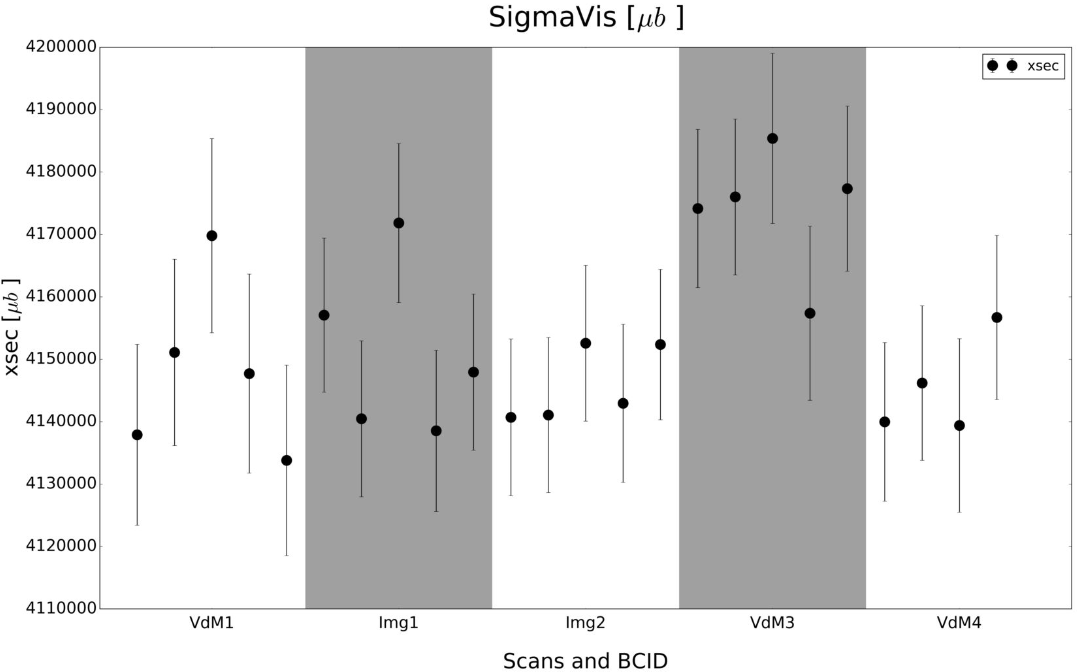
\includegraphics[scale=.25]{Chapter4/DGConst_xsec.png}
    \caption[$\sigma_{vis}$ per BCID for all scans]{ $\sigma_{vis}$ per BCID for all the scans,  in each scan, the BCID's follow the same order, which is 282, 822, 2944, 3123, and 3302.}
    \label{sigmavis_perbcid}
  \end{figure}
\end{center}


Fig \ref{sigmavis_perscan} shows the final  $\sigma_{vis}$ per Scan, which corresponds to the weighted average of the five BCIDs with the weight as: 

\begin{eqnarray}
\frac{1}{\sigma_{vis\text{Err}}^{2}}  \text{     where the error is     } \frac{1}{\sqrt{\sum \frac{1}{\sigma_{vis\text{Err}}^{2}}}}
\label{error}
\end{eqnarray}

After averaging the values of $\sigma_{vis}$ per scan, the error is assigned in the same manner as described in equation (\ref{error}). Figures \ref{sigmavis_perscan} and \ref{sigmavis_perbcid} illustrate that there is a systematic variation in $\sigma_{vis}$ between scans. To account for this, a systematic error is assigned as follows:

\begin{equation}
\sqrt{RMS^{2}-stat^{2}}
\end{equation}

Obtaining a final sigma visible for the calibration $\sigma_{vis}=4163 \pm 3 \text{(stat.)} \pm 12 \text{(syst.)} \text{ mb}$. This result will be useful for a precise luminosity measurement analysis for Run 3 in the CMS experiment of LHC.

\begin{center}
  \begin{figure}[ht]
    \centering
    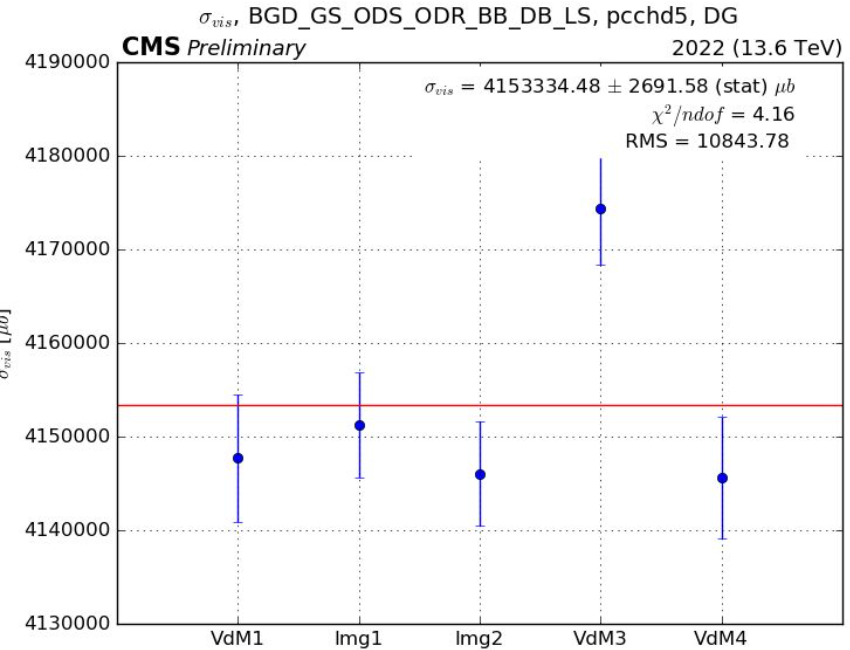
\includegraphics[scale=0.37]{Chapter4/xsec_perscan_v2.png}
    \caption[$\sigma_{vis}$ per Scan]{ $\sigma_{vis}$  per scan.} 
    \label{sigmavis_perscan}
  \end{figure}
\end{center}



